\documentclass{book}

\usepackage[a4paper,margin=3cm]{geometry}
\usepackage{cite} % for IEEE-style citations
\usepackage{listings}
\usepackage{xcolor}
\usepackage[hidelinks]{hyperref}
\usepackage{graphicx}
\usepackage{setspace}
\usepackage{tcolorbox}
\usepackage{tikz}
\usepackage[strings]{underscore}
\usepackage{float}
\usepackage[utf8]{inputenc}  
\usepackage{pmboxdraw}

\usetikzlibrary{trees}

\renewcommand{\contentsname}{Daftar Isi}
\renewcommand{\chaptername}{Bab}

% Define Python language style for listings
\lstdefinestyle{PythonStyle}{
    language=Python,
    basicstyle=\ttfamily\footnotesize,
    keywordstyle=\color{blue}\bfseries,
    commentstyle=\color{gray}\itshape,
    stringstyle=\color{red},
    showstringspaces=false,
    breaklines=true,
    frame=lines,
    numbers=left,
    numberstyle=\tiny\color{gray},
    backgroundcolor=\color{lightgray!10},
    tabsize=4,
    captionpos=b
}

\lstdefinestyle{sql}{
	language=sql,
	keywords={use, insert, into, values, select, from,
	update, set, delete, create, where, join, left, right, inner, order, by, primary, key},
	ndkeywords={max, min, varchar, int},
	ndkeywordstyle=\color{purple}\bfseries,
	basicstyle=\ttfamily\footnotesize,
	keywordstyle=\color{blue},
	commentstyle=\color{gray},
	stringstyle=\color{red},
	breaklines=true,
	showstringspaces=false,
	tabsize=2,
	captionpos=b,
	numbers=left,
	numberstyle=\tiny\color{gray},
	frame=lines,
	backgroundcolor=\color{lightgray!10},
	comment=[l]{\#},
	morecomment=[s]{/*}{*/},
	commentstyle=\color{gray}\ttfamily,
	string=[s]{'}{'},
	morestring=[s]{"}{"},
	%	stringstyle=\color{teal}\ttfamily,
	%	showstringspaces=false
}

\begin{document}
		
	\begin{titlepage}
		\centering
		\vspace*{1cm}
		
		\Huge
		\textbf{IF120203 - Modul Praktikum Pemrograman Dasar}
		
		\vspace{0.5cm}
		
		\LARGE
		Universitas Pradita
		
		\vspace{1.5cm}
		
		\textit{Powered by ChatGPT}
		
		\vspace{2cm}
		
		\textbf{Alfa Yohannis, Ariya Panna}
		
		\vspace{0.8cm}
		
		\today
		
		\vfill
	\end{titlepage}
	
	% Contents Page
	\tableofcontents

	\chapter{Pendahuluan}

\section{Sejarah Pemrograman dan Python}

Pemrograman komputer dimulai pada abad ke-19 dengan penemuan mesin analitik oleh Charles Babbage dan program pertama yang ditulis oleh Ada Lovelace. Sejak itu, pemrograman telah berkembang pesat dengan munculnya bahasa-bahasa pemrograman awal seperti Fortran, COBOL, dan Lisp pada tahun 1950-an. Pada tahun 1970-an dan 1980-an, bahasa pemrograman seperti C, Pascal, dan Basic memperkenalkan konsep-konsep baru dalam pemrograman. Kini, berbagai bahasa pemrograman modern seperti Python, JavaScript, dan Rust digunakan dalam berbagai aplikasi.

Python merupakan bahasa pemrograman \textit{high-level} serbaguna yang pertama kali diperkenalkan pada tahun 1991 oleh Guido van Rossum (GvR). Bahasa ini dirancang agar mudah dipahami dan memiliki struktur kode yang jelas (\textit{readable}), serta mendukung fitur penanganan kesalahan (\textit{exception handling}). Dengan tujuan tersebut, Python berhasil berkembang menjadi bahasa pemrograman yang dapat dimanfaatkan di berbagai bidang. Python merupakan bahasa pemrograman multi-paradigma, yang artinya dapat menggunakan gaya/metode beragam dalam penulisan kode. Saat ini, Python banyak digunakan untuk pengembangan aplikasi web (\textit{server-side}), analisis data, hingga penerapan kecerdasan buatan dan pembelajaran mesin (\textit{machine learning}).
\section{Instalasi di Windows}

Untuk menginstal Python di Windows, ikuti langkah-langkah berikut:

\begin{enumerate}
\item Unduh installer Python terbaru dari situs resmi \href{https://www.python.org/downloads/}{python.org}.
\item Jalankan file installer \texttt{.exe} dan ikuti petunjuk untuk menyelesaikan instalasi.
\item Saat instalasi, centang opsi \textbf{``Add Python to PATH''} agar Python otomatis dikenali di Command Prompt.
\item Ikuti petunjuk instalasi hingga selesai.
\item Verifikasi instalasi dengan membuka Command Prompt lalu ketik:
\begin{verbatim}
    python --version
    pip --version
\end{verbatim}
\end{enumerate}

\section{Instalasi di macOS}

Untuk menginstal Python di macOS, ikuti langkah-langkah berikut:

\begin{enumerate}
\item Unduh installer Python terbaru dari \href{https://www.python.org/downloads/macos/}{python.org}.
\item Jalankan file installer \texttt{.pkg} dan ikuti petunjuk hingga selesai.
\item Alternatif lain, Anda bisa menggunakan Homebrew dengan menjalankan perintah berikut di Terminal:
\begin{verbatim}
    brew install python
\end{verbatim}
\item Setelah instalasi selesai, verifikasi dengan perintah:
\begin{verbatim}
    python3 --version
    pip3 --version
\end{verbatim}
\end{enumerate}

\section{Instalasi di Linux}

Untuk menginstal Python di Linux, ikuti langkah-langkah berikut:

\begin{enumerate}
\item Buka terminal dan jalankan perintah berikut untuk memastikan repositori diperbarui dan Python terpasang:
\begin{verbatim}
    sudo apt update
    sudo apt install python3 python3-pip
\end{verbatim}
\item Verifikasi instalasi dengan perintah:
\begin{verbatim}
    python3 --version
    pip3 --version
\end{verbatim}
\end{enumerate}

\section{IDE dan Editor untuk Python}

\subsection{Apa Itu IDE?}

Integrated Development Environment (IDE) adalah perangkat lunak yang menyediakan fasilitas lengkap untuk pengembangan perangkat lunak. IDE umumnya mencakup editor kode, kompiler atau interpreter, debugger, dan alat manajemen proyek. IDE dirancang untuk mempermudah proses pengembangan perangkat lunak dengan menyediakan antarmuka pengguna yang terintegrasi dan alat-alat yang mendukung pengkodean, pengujian, dan debugging.

Dalam praktikum Python, terdapat beberapa pilihan IDE atau editor yang bisa digunakan, antara lain Visual Studio Code, IDLE (editor bawaan Python), dan PyCharm. Namun, Anda dapat menggunakan IDE atau editor lain yang Anda sukai. Modul praktikum ini menggunakan Visual Studio Code sebagai contoh.

\subsection{Cara Menginstal Visual Studio Code}

\begin{enumerate}
    \item Unduh installer VS Code dari situs resmi \url{https://code.visualstudio.com/}.
    \item Pilih installer sesuai sistem operasi Anda (Windows, macOS, atau Linux).
    \item Jalankan file installer dan ikuti petunjuk instalasi.
    \item Setelah instalasi selesai, buka aplikasi VS Code.
    \item Untuk mendukung pemrograman Python, instal ekstensi \textbf{Python} dari Microsoft melalui menu Extensions (ikon kotak di sidebar kiri).
    \item Untuk membuat file Python, buka menu File (ikon kotak di sidebar kiri) lalu pilih New File (ikon kotak di sidebar kiri) dan ketik nama file yang diinginkan diakhiri dengan \texttt{.py}. Contoh \texttt{hello.py}.
    \item Sekarang Anda dapat mulai menulis dan menjalankan kode Python di dalam VS Code.
\end{enumerate}

\section{Kode Python: hello_world.py}\label{sec:hello_world_code}

\begin{lstlisting}[style=PythonStyle, caption={Kode Python: hello_world.py}]
print("Hello World!")
\end{lstlisting}

Kode di atas merupakan program Python sederhana yang mencetak "Hello World!" ke konsol. Berikut penjelasan dari setiap bagian kode tersebut:

\begin{itemize}
\item \texttt{print(...)} – \texttt{print} adalah fungsi bawaan (\textit{built-in function}) di Python yang digunakan untuk menampilkan output ke layar atau konsol.
\item \texttt{"Hello World!"} – Merupakan sebuah string (teks) yang ditulis di dalam tanda kutip ganda. Nilai string ini akan menjadi argumen yang dikirim ke fungsi \texttt{print}.
\end{itemize}

\section{Panduan Menjalankan Program Python}

Untuk menjalankan program Python di atas, ikuti langkah-langkah berikut:

\begin{enumerate}
	\item Buka terminal atau command prompt.
	\item Navigasikan ke direktori tempat file `hello_world.py` disimpan.
	\begin{verbatim}
		cd /path/ke/direktori
	\end{verbatim}
	\item Jalankan perintah berikut untuk mengkompilasi program:
	\begin{verbatim}
		python hello_world.py
	\end{verbatim}
	\item Jika tidak ada error, program akan dijalankan dan menampilkan "Hello World!" di konsol.
\end{enumerate}

\section{Kode Python: hello_with_input.py}

\begin{lstlisting}[style=PythonStyle, caption={Kode Python: hello_with_input.py}]
nama = input("Masukkan nama Anda: ") # Menerima input dari pengguna

print("Hello " + nama + "!") # Menampilkan output dengan input pengguna
\end{lstlisting}

Berikut penjelasan dari setiap bagian kode tersebut:

\begin{itemize}
\item \texttt{nama = input("Masukkan nama Anda: ")} - Fungsi input merupakan \textit{built-in function} yang digunakan untuk menerima input pengguna dari konsol. Fungsi ini menunda eksekusi program sampai pengguna memasukkan input dan menampilkan opsional pesan untuk meminta input yang kemudian disimpan dalam variabel \texttt{nama}.
\item \texttt{print("Hello " + nama + " !")} - Seperti yang dijelaskan pada Section~\ref{sec:hello_world_code}, fungsi print digunakan untuk mencetak output ke layar atau konsol. Di sini, pesan "Hello [Nama]!" diisi dengan input pengguna.
\end{itemize}


\section{Latihan}

Berikut adalah beberapa latihan yang dapat Anda coba untuk memperdalam pemahaman tentang program Python yang telah dibahas:

\begin{enumerate}
\item \label{sec:first-exercise} \textbf{Latihan 1:} Buat file baru dengan nama \textbf{introduction.py} yang dimana program harus menerima input nama, usia, dan domisili dari pengguna kemudian mencetak pesan dengan format yang ditentukan
\begin{lstlisting}[style=PythonStyle, caption={Latihan 1}]
nama = input("Masukkan nama Anda: ")
prodi = input("Masukkan program studi Anda: ")
angkatan = input("Masukkan angkatan Anda: ")

print("Halo! Nama saya " + nama + ". Saya mahasiswa program studi " + prodi + " tahun angkatan " + angkatan + ".")
\end{lstlisting}

Contoh input dan output yang diberikan ketika program dijalankan:

\begin{verbatim}
Input:
Masukkan Nama Anda: Bob Smith
Masukkan Program Studi Anda: Informatika
Masukkan Tahun Angkatan: 2025

Output:
Halo! Nama saya Bob Smith. Saya mahasiswa program studi Informatika tahun angkatan 2025.
\end{verbatim}

\item \textbf{Latihan 2:} Latihan ini bertujuan untuk belajar memformat teks (\textit{string}) menggunakan \textbf{f-string}, membuat output lebih rapi tanpa perlu menggunakan operator \texttt{+} sebagai penghubung antara teks. Buat file baru dengan nama \textbf{introduction_with_fstring.py} dan isinya mirip dengan \hyperref[sec:first-exercise]{Latihan 1}, namun format outputnya menggunakan \textbf{f-string}

\begin{lstlisting}[style=PythonStyle, caption={Latihan 2}]
nama = input("Masukkan nama Anda: ")
prodi = input("Masukkan program studi Anda: ")
angkatan = input("Masukkan angkatan Anda: ")

print(f"Halo! Nama saya {nama}. Saya mahasiswa program studi {prodi} tahun angkatan {angkatan}. Output dihasilkan menggunakan f-string")
\end{lstlisting}

Contoh input dan output yang diberikan ketika program dijalankan:

\begin{verbatim}
Input:
Masukkan Nama Anda: Bob Smith
Masukkan Program Studi Anda: Informatika
Masukkan Tahun Angkatan: 2025

Output:
Halo! Nama saya Bob Smith. Saya mahasiswa program studi Informatika tahun angkatan 2025. 
Output dihasilkan menggunakan f-string
\end{verbatim}

\item \textbf{Latihan 3:} \textit{Escape Character} merupakan karakter khusus yang digunakan (biasanya diawali dengan \texttt{\textbackslash}) yang digunakan di dalam string untuk mengatur penataan teks atau menampilkan karakter spesial. Dengan escape character, kita bisa:

\begin{itemize}
    \item Membuat teks pindah baris: \texttt{\textbackslash n}
    \item Menambahkan tabulasi: \texttt{\textbackslash t}
    \item Menulis tanda kutip di dalam string: \texttt{\textbackslash "}
    \item Menampilkan backslash asli: \texttt{\textbackslash\textbackslash}
\end{itemize}

Buat file baru dengan nama \textbf{escape_character.py} dan isinya seperti berikut:

\begin{lstlisting}[style=PythonStyle, caption={Latihan 3}]
print("Hello\nWorld") # Membuat teks pindah baris
print("Hello\tWorld") # Menambahkan tabulasi
print("Hello \"World") # Menulis tanda kutip di dalam string
print("Hello \\ World") # Menampilkan backslash asli
\end{lstlisting}

Output yang akan dihasilkan dari program di atas adalah:

\begin{verbatim}
Hello
World
Hello	World
Hello "World
Hello \ World
\end{verbatim}
\end{enumerate}

\section{Soal Latihan}

Berikut adalah beberapa soal latihan tambahan untuk menguji pemahaman Anda mengenai konsep yang telah dipelajari:

\begin{enumerate}
\item \textbf{Soal 1:} Buat program bernama \texttt{biodata.py} yang meminta input berupa:
\begin{itemize}
	\item Nama lengkap
	\item Umur
	\item Hobi
\end{itemize}
	Cetak output dengan format berikut menggunakan \textbf{f-string}. Berikut merupakan contoh input dan output yang diharapkan:
\begin{verbatim}
Input:
Masukkan Nama Lengkap: Jane Hopkins
Masukkan Usia Anda: 20
Masukkan Hobi Anda: Ngoding

Output:
Halo, nama saya Jane Hopkins. Saya berusia 20 tahun dan hobi saya adalah Ngoding.
\end{verbatim}

\item \textbf{Soal 2:}  
Buat program bernama \texttt{quote.py} yang menampilkan kutipan favoritmu. Gunakan \textbf{escape character} untuk menampilkan tanda kutip di dalam string. Contoh output:

\begin{verbatim}
Input:
Masukkan kutipan favoritmu dari Albert Einstein: "Imagination is more important 
than knowledge."

Output:
Kata Albert Einstein: "Imagination is more important than knowledge."
\end{verbatim}

\item \textbf{Soal 3:} Buat program bernama \texttt{schedule.py} yang menampilkan jadwal kuliah. Gunakan \textbf{tabulasi} (\texttt{\textbackslash t}) untuk merapikan kolom. Contoh output:

\begin{tabular}{l l l}
    \textbf{Hari} & \textbf{Waktu} & \textbf{Mata Kuliah} \\
    Senin & 07.00 & Algoritma \\
    Selasa & 09.00 & Basis Data \\
    Selasa & 13.00 & Pemrograman Dasar \\
\end{tabular}
\end{enumerate}

	\chapter{Variabel, Konstanta, Tipe Data Dasar, dan Konversi Tipe Data}

\section{Variabel}

Variabel merupakan tempat penyimpanan sementara yang digunakan untuk menampung data selama program berjalan, sehingga data tersebut dapat digunakan kembali. Berbeda dengan bahasa pemrograman \textit{static type} seperti C, C++, dan Java yang harus secara eksplisit menulis tipe data untuk variabel. Di Python, variabel memiliki tipe data yang dinamis (\textit{dynamic type}) dan dapat berubah sesuai dengan kebutuhan program.
\newline

\begin{figure}[H]
	\centering
	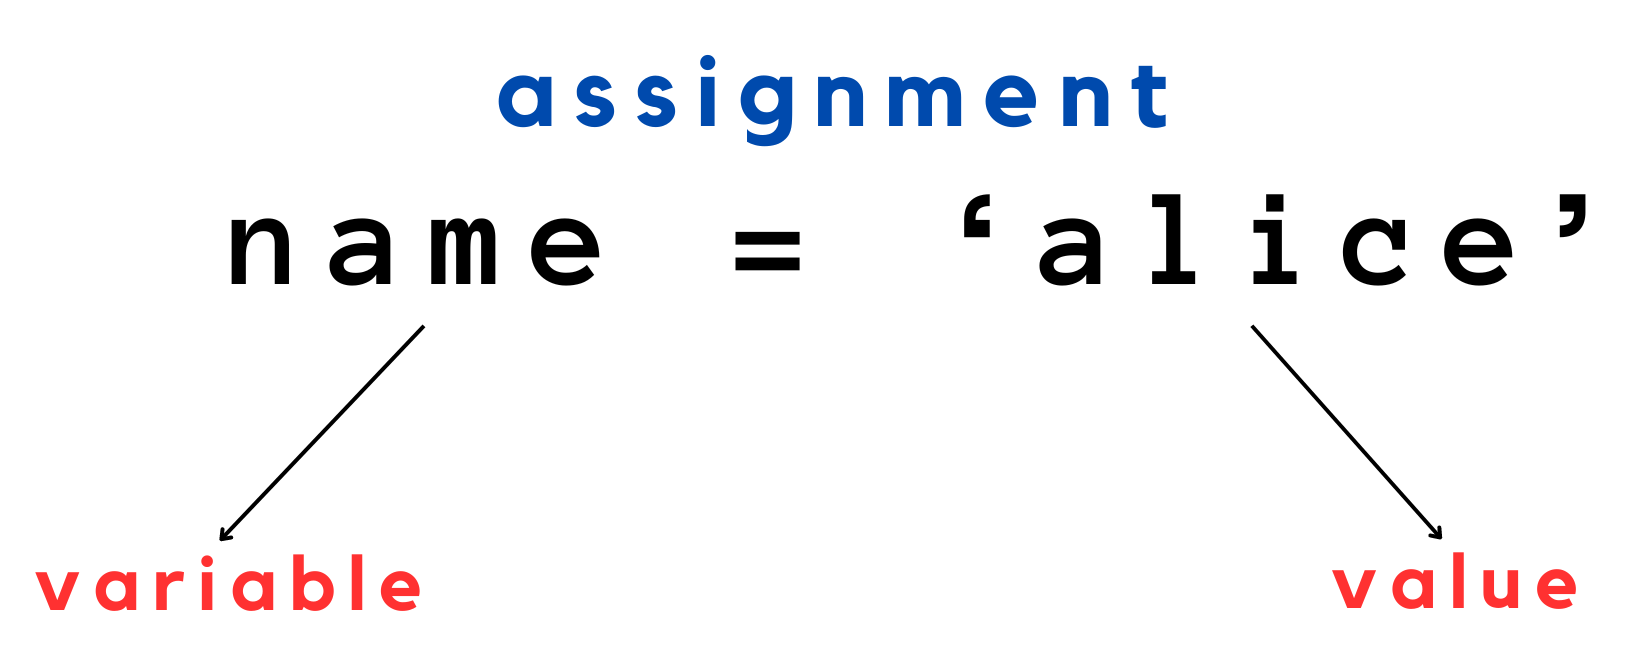
\includegraphics[width=0.7\textwidth]{../shared_assets/images/python_variable_structure.png}
	\caption{Struktur Variabel di Python}
	\label{fig:python-variable-structure}
\end{figure}

\noindent
Sumber gambar: \url{https://www.packetswitch.co.uk/python-variables-data-types/}

\subsection{Aturan Penamaan Variabel}

Pemberian nama variabel di Python harus mematuhi beberapa aturan penamaan yang disediakan oleh Python. Berikut adalah beberapa aturan penamaan variabel di Python:

\begin{itemize}
	\item Nama variabel harus dimulai dengan huruf atau underscore (\_).
	\item Nama variabel tidak boleh dimulai dengan angka.
	\item Nama variabel tidak boleh mengandung spasi.
	\item Nama variabel tidak boleh mengandung simbol.
	\item Nama variabel tidak boleh mengandung kata kunci (\textit{keyword}) yang sudah terdefinisi dalam Python, seperti \texttt{def}, \texttt{for}, \texttt{if}, \texttt{return}, dan sebagainya.
\end{itemize}

\subsection{Latihan Membuat Variabel}

Buat file baru dengan nama \textbf{variable.py} dan buat variabel dengan nama \textbf{nama}, \textbf{usia}, dan \textbf{berat_badan} dengan tipe data yang sesuai dan nilai-nilai yang sesuai. Kemudian cetak variabel tersebut.

\begin{lstlisting}[style=PythonStyle, caption={Kode Python: variable.py}]
nama = "Stefani Laurensia"
usia = 21
berat_badan = 50.2

print(nama)
print(usia)
print(berat_badan)
\end{lstlisting}

\subsection{Contoh Kesalahan Penamaan Variabel}

\begin{lstlisting}[style=PythonStyle, caption={Kode Python: variable.py}]
1angka = 200 # Nama variabel tidak boleh dimulai dengan angka
nama lengkap = "Budi" # Nama variabel tidak boleh mengandung spasi
gaji$ = 1000000 # Nama variabel tidak boleh mengandung simbol
class = "Informatika" # class merupakan kata kunci untuk membuat sebuah class di Python sehingga melanggar aturan di mana nama variabel tidak boleh mengandung kata kunci
\end{lstlisting}

\section{Konstanta}

Konstanta adalah variabel yang seharusnya nilainya tidak berubah selama program berjalan. Contohnya nilai \textbf{\textit{pi}} (3.14) atau gravitasi (9.81). Di Python, kita bisa menandai variabel sebagai Final dari modul \texttt{typing} untuk memberi tanda bahwa variabel tersebut dimaksudkan sebagai konstanta. Namun ada hal-hal yang perlu diperhatikan:
\begin{itemize}
	\item Python tidak memaksa variabel \texttt{Final} agar tidak bisa diubah.
	\item Penandaan \texttt{Final} hanya \textbf{memberi peringatan pada type checker}, bukan mencegah perubahan di runtime.
\end{itemize}

\subsection{Aturan Penamaan Konstanta}

Untuk menandakan bahwa sebuah variabel adalah konstanta, kita bisa menggunakan huruf besar untuk membedakan dengan variabel biasa. Hal ini mengikuti aturan penamaan variabel yang dibuat oleh Python (\href{https://peps.python.org/pep-0008/}{PEP 8 - Style Guide for Python Code}).

\subsection{Latihan Membuat Konstanta}

Buat file baru dengan nama \textbf{constant.py} dan buat konstanta dengan nama \textbf{PI} dan \textbf{GRAVITASI} dengan nilai yang sesuai. Kemudian cetak konstanta tersebut. Namun, berbeda dari bahasa pemrograman lain seperti C, C++, atau Java, di Python konstanta dapat diubah.
\begin{lstlisting}[style=PythonStyle, caption={Kode Python: constant.py}]
from typing import Final

PI: Final = 3.14
GRAVITASI: Final = 9.81

print(PI)
print(GRAVITASI)

GRAVITASI = 10 # Nilai masih tetap bisa berubah, tapi tidak disarankan
print(GRAVITASI)
\end{lstlisting}

\section{Tipe Data Dasar}

Tipe data merupakan jenis data yang bisa disimpan di program Python. Tipe data di Python memiliki banyak jenis, seperti \texttt{int}, \texttt{float}, \texttt{str}, \texttt{bool}, \texttt{list}, \texttt{tuple}, \texttt{dict}, dan \texttt{set}. Namun pada \textit{chapter} kali ini, kita akan fokus pada tipe data dasar, antara lain \texttt{int}, \texttt{float}, \texttt{str}, dan \texttt{bool}.
\newline \newline
Berdasarkan kelompoknya, tipe data dasar di Python dapat dibedakan menjadi 3 kelompok, antara lain:

\begin{enumerate}
\item \textbf{Numeric} (Angka)
\begin{enumerate}
\item \textbf{Integer} (bilangan bulat)
\begin{lstlisting}[style=PythonStyle]
usia = 18
jumlah_mahasiswa = 64
nomor_rumah = 88

suhu = -5
\end{lstlisting}

\item \textbf{Float} (bilangan desimal)
\begin{lstlisting}[style=PythonStyle]
koordinat_x = 5.5
koordinat_y = 7.8

saldo = 10.500.075
\end{lstlisting}
\end{enumerate}

\item \textbf{Teks} (Kata / Kalimat)
\begin{enumerate}
\item \textbf{String} (kumpulan karakter)
\begin{lstlisting}[style=PythonStyle]
nama = "John"
quote = 'Programmer: A machine that turns coffee into code'
pesan_email = """
Kepada Yth. John Doe,

Terima kasih atas pesanan anda.
"""
\end{lstlisting}
\end{enumerate}

\item \textbf{Boolean} (Benar atau Salah)
\begin{lstlisting}[style=PythonStyle]
is_married = False
is_single = True
\end{lstlisting}
\end{enumerate}

\section{Konversi Tipe Data (\textit{Type Casting})}

Kadang kita perlu mengubah tipe data dari satu jenis ke jenis lain agar Python bisa memprosesnya dengan benar.
Misal, input dari pengguna melalui fungsi \texttt{input()} selalu mengembalikan tipe data string (str), tapi kita ingin melakukan perhitungan angka, maka kita harus mengubahnya menjadi int atau float.

\begin{table}[h!]
\centering
\begin{tabular}{|c|c|c|}
\hline
\textbf{Fungsi} & \textbf{Keterangan} & \textbf{Contoh} \\
\hline
int() & Ubah menjadi bilangan bulat & int("10") → 10 \\
\hline
float() & Ubah menjadi bilangan desimal & float("3.14") → 3.14 \\
\hline
str() & Ubah menjadi teks & str(10) → "10" \\
\hline
bool() & Ubah menjadi True/False & bool(0) → False, bool(5) → True \\
\hline
\end{tabular}
\caption{Fungsi Untuk Konversi Tipe Data di Python}
\end{table}

\subsection{Latihan Konversi Tipe Data}

\begin{lstlisting}[style=PythonStyle, caption={Kode Python: string_to_int.py}]
usia = input("Masukkan usia Anda: ")
print("Tipe data sebelum konversi:", type(usia)) # Menampilkan tipe data sebelum konversi

usia = int(usia) # Konversi tipe data string menjadi integer
print("Tipe data setelah konversi:", type(usia)) # Menampilkan tipe data setelah konversi

usia_lima_tahun_kemudian = usia + 5 # Perhitungan usia 5 tahun kemudian
print("Usia 5 tahun kemudian:", usia_lima_tahun_kemudian)
\end{lstlisting}

\begin{lstlisting}[style=PythonStyle, caption={Kode Python: string_to_float.py}]
angka_str = "45.67"
print("Sebelum konversi:", angka_str, type(angka_str))

angka_float = float(angka_str)
print("Setelah konversi ke float:", angka_float, type(angka_float))
\end{lstlisting}

\begin{lstlisting}[style=PythonStyle, caption={Kode Python: int_to_float.py}]
angka_int = 10
print("Sebelum konversi:", angka_int, type(angka_int))

angka_float = float(angka_int)
print("Setelah konversi ke float:", angka_float, type(angka_float))
\end{lstlisting}

\begin{lstlisting}[style=PythonStyle, caption={Kode Python: float_to_int.py}]
angka_float = 3.99
print("Sebelum konversi:", angka_float, type(angka_float))

angka_int = int(angka_float)
print("Setelah konversi ke integer:", angka_int, type(angka_int))
\end{lstlisting}

\subsection{Kesalahan dalam Konversi Tipe Data}
Meskipun Python menyediakan fungsi bawaan untuk mengubah tipe data (\texttt{int()}, \texttt{float()}, \texttt{str()}, \texttt{bool()}), \textbf{tidak semua konversi bisa dilakukan dengan sukses}. Jika nilai yang dikonversi tidak sesuai dengan tipe data tujuan, maka program akan menghasilkan \textbf{error}. Berikut adalah contoh kesalahan dalam konversi tipe data:

\begin{lstlisting}[style=PythonStyle]
# String huruf → Integer
huruf = "abc"
huruf_integer = int(huruf) 
# Output: ValueError: invalid literal for int() with base 10: 'abc'

# String bilangan desimal → Integer
angka_str = "12.34"
angka_int = int(angka_str)  
# Output: ValueError: invalid literal for int() with base 10: '12.34'
\end{lstlisting}

Perhatikan pada contoh di atas bahwa program akan menghasilkan \textbf{error} ketika nilai yang dikonversi tidak sesuai dengan tipe data tujuan. Hal ini diakibatkan karena fungsi \texttt{int()} hanya dapat mengubah \textbf{string yang berisi bilangan bulat} menjadi tipe data \texttt{integer}.
\par
Apabila string berisi karakter non-angka (misalnya \texttt{"abc"}) atau bilangan desimal (misalnya \texttt{"12.34"}), maka Python tidak dapat memprosesnya langsung sebagai \texttt{integer} dan akan menampilkan pesan \texttt{ValueError}. Untuk kasus bilangan desimal dalam bentuk string, diperlukan dua tahap konversi, yaitu:
\begin{enumerate}
	\item Konversi string ke tipe data \texttt{float}.
	\item Konversi tipe data \texttt{float} ke tipe data \texttt{integer}.
\end{enumerate}

\section{Soal Latihan}

Berikut adalah beberapa soal latihan tambahan untuk menguji pemahaman Anda mengenai konsep variabel, konstanta tipe data, dan konversi tipe data yang telah dipelajari:
\begin{enumerate}
\item \textbf{Soal 1:} Buat program bernama \texttt{luas_persegi_panjang.py} yang meminta pengguna memasukan nilai panjang dan lebar persegi panjang, kemudian program harus bisa menghitung dan mencetak luas persegi panjang tersebut.
\newline \newline
\textbf{Hint:} Gunakan operator perkalian \texttt{*} untuk menghitung luas.

\item \textbf{Soal 2:} Buat program bernama \texttt{luas_lingkaran.py} yang meminta pengguna memasukan nilai jari-jari lingkaran. Program harus menampung nilai konstanta \textbf{\textit{pi}} mengikuti standar \textit{best practice} dari Python dan bisa menghitung sekaligus mencetak luas lingkaran tersebut.

\item \textbf{Soal 3:} Buat program bernama \texttt{tebak_usia.py} yang meminta pengguna memasukkan tahun lahirnya. Program harus:
\begin{enumerate}
    \item Menyimpan tahun lahir di variabel.
    \item Mengubah input dari string menjadi integer.
    \item Menghitung umur dengan mengurangi tahun saat ini dengan tahun lahir yang dimasukan oleh pengguna.
    \item Menampilkan pesan seperti: "Kamu berusia [umur] tahun."
\end{enumerate}

\textbf{Hint:} Gunakan operator pengurangan \texttt{-} untuk menghitung usia saat ini.

\end{enumerate}
	\chapter{Operator dan Pengkondisian}

\section{Operator}
Operator adalah karakter khusus yang digunakan untuk melakukan operasi terhadap variabel dan nilai. Di Python terdapat berbagai jenis operator, namun pada chapter ini kita hanya akan membahas beberapa operator yang paling umum digunakan, yaitu:

\begin{enumerate}
    \item Operator Aritmatika
    \item Operator \textit{Assignment}
    \item Operator Perbandingan
    \item Operator Logika
    \item Operator \textit{Membership}
\end{enumerate}

\subsection{Operator Aritmatika}
\begin{frame}[fragile]{Operator Aritmatika di Python}
Operator ini dipakai untuk melakukan operasi dasar dalam matematika, seperti penjumlahan, pengurangan, perkalian, pembagian, dan sebagainya.

\end{frame}

\begin{table}[H]
\centering
\begin{tabular}{|c|c|c|}
\hline
\textbf{Operator} & \textbf{Keterangan} \\
\hline
\texttt{+} & Operator penjumlahan \\
\hline
\texttt{-} & Operator pengurangan \\
\hline
\texttt{*} & Operator perkalian \\
\hline
\texttt{/} & Operator pembagian \\
\hline
\texttt{//} & Operator pembagian bulat (\textit{floor division}) \\
\hline
\texttt{\%} & Operator modulus (sisa hasil bagi) \\
\hline
\texttt{**} & Operator perpangkatan \\
\hline
\end{tabular}
\caption{Daftar Operator Aritmatika di Python}
\end{table}

Berikut adalah contoh penggunaan operator aritmatika dalam Python:
\begin{lstlisting}[style=PythonStyle, caption={Kode Python: arithmetic_operator.py}]
a = 5
b = 2

print("a + b =", a + b)
print("a - b =", a - b)
print("a * b =", a * b)
print("a / b =", a / b)
print("a // b =", a // b)
print("a % b =", a % b)
print("a ** b =", a ** b)
\end{lstlisting}

Kode di atas mendemonstrasikan berbagai operasi aritmatika yang dapat dilakukan di Python menggunakan operator bawaan. Berikut adalah penjelasan dari setiap operasi:
\begin{itemize}
    \item Penjumlahan (+)
    \begin{itemize}
        \item \texttt{print("a + b =", a + b)} menghasilkan penjumlahan dari \texttt{a} dan \texttt{b}, yaitu $5 + 2 = 7$.
    \end{itemize}

    \item Pengurangan (-)
    \begin{itemize}
        \item \texttt{print("a - b =", a - b)} menghasilkan pengurangan dari \texttt{a} dan \texttt{b}, yaitu $5 - 2 = 3$.
    \end{itemize}

    \item Perkalian (*)
    \begin{itemize}
        \item \texttt{print("a * b =", a * b)} menghasilkan perkalian dari \texttt{a} dan \texttt{b}, yaitu $5 \times 2 = 10$.
    \end{itemize}

    \item Pembagian (/)
    \begin{itemize}
        \item \texttt{print("a / b =", a / b)} menghasilkan pembagian dari \texttt{a} dan \texttt{b}, yaitu $5 / 2 = 2.5$.
    \end{itemize}

    \item \textit{Floor Division} (//)
    \begin{itemize}
        \item \texttt{print("a // b =", a // b)} menghasilkan pembagian bulat dari \texttt{a} dan \texttt{b} dengan pembulatan ke bawah, yaitu $5 // 2 = 2$.
    \end{itemize}

    \item Modulo (\%)
    \begin{itemize}
        \item \texttt{print("a \% b =", a \% b)} menghasilkan sisa hasil bagi dari \texttt{a} dibagi \texttt{b}, yaitu $5 \% 2 = 1$.
    \end{itemize}

    \item Perpangkatan (**)
    \begin{itemize}
        \item \texttt{print("a ** b =", a ** b)} menghasilkan \texttt{a} dipangkatkan dengan \texttt{b}, yaitu $5^2 = 25$.
    \end{itemize}
\end{itemize}

\subsection{Operator \textit{Assignment}}
Operator \textit{assignment} adalah operator yang digunakan untuk memberikan nilai pada variabel. 
Selain \textit{assignment} dasar dengan tanda sama dengan (\texttt{=}), Python juga menyediakan operator 
\textit{assignment} gabungan (\textit{augmented assignment}) yang mengombinasikan operasi aritmatika dengan assignment.

\begin{table}[H]
\centering
\begin{tabular}{|c|c|}
\hline
\textbf{Operator} & \textbf{Keterangan} \\
\hline
\texttt{=} & Assignment, memberikan nilai ke variabel \\
\hline
\texttt{+=} & Penjumlahan sekaligus assignment (\texttt{x += y} $\Rightarrow$ \texttt{x = x + y}) \\
\hline
\texttt{-=} & Pengurangan sekaligus assignment (\texttt{x -= y} $\Rightarrow$ \texttt{x = x - y}) \\
\hline
\texttt{*=} & Perkalian sekaligus assignment (\texttt{x *= y} $\Rightarrow$ \texttt{x = x * y}) \\
\hline
\texttt{/=} & Pembagian sekaligus assignment (\texttt{x /= y} $\Rightarrow$ \texttt{x = x / y}) \\
\hline
\texttt{//=} & Floor division sekaligus assignment (\texttt{x //= y} $\Rightarrow$ \texttt{x = x // y}) \\
\hline
\texttt{\%=} & Modulo sekaligus assignment (\texttt{x \%= y} $\Rightarrow$ \texttt{x = x \% y}) \\
\hline
\texttt{**=} & Perpangkatan sekaligus assignment (\texttt{x **= y} $\Rightarrow$ \texttt{x = x ** y}) \\
\hline
\end{tabular}
\caption{Daftar Operator Assignment di Python}
\end{table}

Berikut adalah contoh penggunaan operator assignment dalam Python:
\begin{lstlisting}[style=PythonStyle, caption={Kode Python: assignment_operator.py}]
x = 10
print("x =", x)

x += 5
print("x += 5 ->", x)

x -= 3
print("x -= 3 ->", x)

x *= 2
print("x *= 2 ->", x)

x /= 4
print("x /= 4 ->", x)

x //= 2
print("x //= 2 ->", x)

x %= 3
print("x %= 3 ->", x)

x **= 2
print("x **= 2 ->", x)
\end{lstlisting}

Kode di atas mendemonstrasikan berbagai operator assignment yang dapat digunakan di Python. 
Berikut adalah penjelasan dari setiap operator:
\begin{itemize}
    \item Assignment (=)
    \begin{itemize}
        \item \texttt{x = 10} memberikan nilai $10$ ke variabel \texttt{x}.
    \end{itemize}

    \item Penjumlahan Assignment (+=)
    \begin{itemize}
        \item \texttt{x += 5} sama dengan \texttt{x = x + 5}. Jika sebelumnya $x = 10$, maka setelah operasi ini $x = 15$.
    \end{itemize}

    \item Pengurangan Assignment (-=)
    \begin{itemize}
        \item \texttt{x -= 3} sama dengan \texttt{x = x - 3}. Jika $x = 15$, maka hasilnya $x = 12$.
    \end{itemize}

    \item Perkalian Assignment (*=)
    \begin{itemize}
        \item \texttt{x *= 2} sama dengan \texttt{x = x * 2}. Jika $x = 12$, maka hasilnya $x = 24$.
    \end{itemize}

    \item Pembagian Assignment (/=)
    \begin{itemize}
        \item \texttt{x /= 4} sama dengan \texttt{x = x / 4}. Jika $x = 24$, maka hasilnya $x = 6.0$.
    \end{itemize}

    \item Floor Division Assignment (//=)
    \begin{itemize}
        \item \texttt{x //= 2} sama dengan \texttt{x = x // 2}. Jika $x = 6.0$, maka hasilnya $x = 3.0$.
    \end{itemize}

    \item Modulo Assignment (\%=)
    \begin{itemize}
        \item \texttt{x \%= 3} sama dengan \texttt{x = x \% 3}. Jika $x = 3.0$, maka hasilnya $x = 0.0$.
    \end{itemize}

    \item Perpangkatan Assignment (**=)
    \begin{itemize}
        \item \texttt{x **= 2} sama dengan \texttt{x = x ** 2}. Jika $x = 0.0$, maka hasilnya tetap $0.0$.
    \end{itemize}
\end{itemize}

\subsection{Operator Perbandingan}
Operator perbandingan digunakan untuk membandingkan dua nilai. 
Hasil dari operator ini selalu berupa nilai boolean (\texttt{True} atau \texttt{False}).

\begin{table}[H]
\centering
\begin{tabular}{|c|c|}
\hline
\textbf{Operator} & \textbf{Keterangan} \\
\hline
\texttt{==} & Sama dengan \\
\hline
\texttt{!=} & Tidak sama dengan \\
\hline
\texttt{>} & Lebih besar dari \\
\hline
\texttt{<} & Lebih kecil dari \\
\hline
\texttt{>=} & Lebih besar atau sama dengan \\
\hline
\texttt{<=} & Lebih kecil atau sama dengan \\
\hline
\end{tabular}
\caption{Daftar Operator Perbandingan di Python}
\end{table}

\begin{lstlisting}[style=PythonStyle, caption={Kode Python: comparison_operator.py}]
a = 5
b = 2

print("a == b:", a == b)
print("a != b:", a != b)
print("a > b:", a > b)
print("a < b:", a < b)
print("a >= b:", a >= b)
print("a <= b:", a <= b)
\end{lstlisting}

\subsection{Operator Logika}
Operator logika digunakan untuk menggabungkan ekspresi boolean.

\begin{table}[H]
\centering
\begin{tabular}{|c|c|}
\hline
\textbf{Operator} & \textbf{Keterangan} \\
\hline
\texttt{and} & Bernilai \texttt{True} jika kedua kondisi bernilai benar \\
\hline
\texttt{or} & Bernilai \texttt{True} jika salah satu kondisi bernilai benar \\
\hline
\texttt{not} & Membalikkan nilai boolean (True menjadi False, sebaliknya) \\
\hline
\end{tabular}
\caption{Daftar Operator Logika di Python}
\end{table}

\begin{lstlisting}[style=PythonStyle, caption={Kode Python: logical_operator.py}]
x = True
y = False

print("x and y:", x and y)
print("x or y:", x or y)
print("not x:", not x)
\end{lstlisting}

\subsection{Operator \textit{Membership}}
Operator \textit{membership} digunakan untuk memeriksa apakah suatu nilai (biasanya berupa karakter atau substring) 
terdapat di dalam sebuah string. Hasil dari operasi ini berupa nilai boolean (\texttt{True} atau \texttt{False}).

\begin{table}[H]
\centering
\begin{tabular}{|c|c|}
\hline
\textbf{Operator} & \textbf{Keterangan} \\
\hline
\texttt{in} & Bernilai \texttt{True} jika nilai ada di dalam string \\
\hline
\texttt{not in} & Bernilai \texttt{True} jika nilai tidak ada di dalam string \\
\hline
\end{tabular}
\caption{Daftar Operator \textit{Membership} di Python}
\end{table}

\begin{lstlisting}[style=PythonStyle, caption={Kode Python: membership_operator.py}]
text = "Python Programming"

print("'Py' in text:", "Py" in text)         # True
print("'Java' in text:", "Java" in text)     # False
print("'Java' not in text:", "Java" not in text) # True
print("'P' in text:", "P" in text)           # True
\end{lstlisting}

\section{Pengkondisian}
Pengkondisian adalah konsep penting dalam pemrograman yang memungkinkan pengambilan keputusan berdasarkan kondisi tertentu. Di Python, pengkondisian bisa diimplementasikan menggunakan beberapa struktur dasar seperti if, elif, else, match, dan operator ternary.

\subsection{If}
If digunakan untuk mengeksekusi blok kode tertentu hanya jika kondisi yang diberikan bernilai true. Bentuk dasarnya adalah:

\begin{lstlisting}[style=PythonStyle, caption={Bentuk dasar if}]
if kondisi:
    # Blok kode yang akan dieksekusi jika kondisi bernilai true
\end{lstlisting}

Contoh Penggunaan:

\begin{lstlisting}[style=PythonStyle, caption={Kode Python: if_statement.py}]
nilai = 75
if nilai >= 70:
    print("Lulus")
\end{lstlisting}

\subsection{If-Else}
If-else memungkinkan kita untuk menentukan blok kode alternatif yang akan dijalankan jika kondisi tidak terpenuhi. Bentuk dasarnya adalah:

\begin{lstlisting}[style=PythonStyle, caption={Bentuk dasar if-else}]
if kondisi:
    # Blok kode yang akan dieksekusi jika kondisi bernilai true
else:
    # Blok kode yang akan dieksekusi jika kondisi bernilai false
\end{lstlisting}

Contoh Penggunaan:

\begin{lstlisting}[style=PythonStyle, caption={Kode Python: if_else_statement.py}]
nilai = 65
if nilai >= 70:
    print("Lulus")
else:
    print("Tidak Lulus")
\end{lstlisting}

\subsection{If-Elif-Else (Percabangan Multi Kondisi)}
If-elif-else memungkinkan kita untuk menentukan beberapa kondisi dan blok kode yang akan dijalankan jika kondisi tersebut bernilai true. Bentuk dasarnya adalah:

\begin{lstlisting}[style=PythonStyle, caption={Bentuk dasar if-elif-else}]
if kondisi1:
    # Blok kode yang akan dieksekusi jika kondisi1 bernilai true
elif kondisi2:
    # Blok kode yang akan dieksekusi jika kondisi2 bernilai true
else:
    # Blok kode yang akan dieksekusi jika kondisi1 dan kondisi2 bernilai false
\end{lstlisting}

Contoh Penggunaan:

\begin{lstlisting}[style=PythonStyle, caption={Kode Python: if_elif_else_statement.py}]
nilai = 65
if nilai >= 90:
    print("A")
elif nilai >= 80:
    print("B")
elif nilai >= 70:
    print("C")
else:
    print("D")
\end{lstlisting}

\subsection{\textit{Nested-If}}
\textit{Nested-if} adalah struktur if yang digunakan untuk membuat blok kode yang bersarang. Bentuk dasarnya adalah:

\begin{lstlisting}[style=PythonStyle, caption={Bentuk dasar nested-if}]
if kondisi1:
    # Blok kode yang akan dieksekusi jika kondisi1 bernilai true
    if kondisi2:
        # Blok kode yang akan dieksekusi jika kondisi2 bernilai true
    else:
        # Blok kode yang akan dieksekusi jika kondisi2 bernilai false
else:
    # Blok kode yang akan dieksekusi jika kondisi1 bernilai false
\end{lstlisting}

Contoh Penggunaan:

\begin{lstlisting}[style=PythonStyle, caption={Kode Python: nested_if_statement.py}]
usia = 25
punya_surat_izin_mengemudi = True

if usia >= 18:  # Kondisi luar: cek apakah usia sudah 18 tahun ke atas
    print("Kamu sudah dewasa.")
    if punya_surat_izin_mengemudi:  # Kondisi dalam: cek apakah sudah punya SIM
        print("Kamu boleh mengemudi.")
    else:
        print("Kamu sudah dewasa, tapi belum punya SIM.")
else:
    print("Kamu belum dewasa.")
\end{lstlisting}

\subsection{\textit{Match}}
Sejak Python 3.10, tersedia struktur kontrol baru bernama \texttt{match} yang mirip dengan \texttt{switch-case} di bahasa pemrograman lain. Dengan \texttt{match}, kita dapat mencocokkan sebuah nilai terhadap beberapa pola sekaligus. Bentuk dasarnya adalah:

\begin{lstlisting}[style=PythonStyle, caption={Bentuk dasar match}]
match variabel / value:
    case pola1:
        # blok kode jika sesuai pola1
    case pola2:
        # blok kode jika sesuai pola2
    case _:
        # blok kode default jika tidak ada yang cocok
\end{lstlisting}

Berikut contoh penggunaannya:

\begin{lstlisting}[style=PythonStyle, caption={Kode Python: match.py}]
hari = "Senin"

match hari:
    case "Senin":
        print("Awal minggu, semangat kerja!")
    case "Jumat":
        print("Akhir minggu, hampir libur!")
    case _:
        print("Hari biasa.")
\end{lstlisting}

\subsection{Operator Ternary (\textit{Conditional Expression})}

Python mendukung bentuk singkat dari struktur \texttt{if-else} yang disebut dengan
\textit{conditional expression} atau sering dikenal sebagai \textit{ternary operator}.
Sintaksnya adalah:

\begin{lstlisting}[style=PythonStyle, caption={Bentuk dasar ternary operator di Python}]
nilai_jika_true if kondisi else nilai_jika_false
\end{lstlisting}

Contoh penggunaannya:

\begin{lstlisting}[style=PythonStyle, caption={Kode Python: ternary_operator.py}]
usia = 20

status = "Dewasa" if usia >= 18 else "Anak-anak"

print("Status:", status)
\end{lstlisting}

Kode di atas setara dengan:

\begin{lstlisting}[style=PythonStyle]
if usia >= 18:
    status = "Dewasa"
else:
    status = "Anak-anak"
\end{lstlisting}

\section{Latihan}
Berikut adalah beberapa latihan yang dapat Anda coba untuk memperdalam pemahaman tentang program Python yang telah dibahas:

\begin{enumerate}
\item \textbf{Latihan 1:} Buatlah program yang menerima input 5 nilai asesmen mahasiswa yang kemudian dihitung rata-ratanya. Berdasarkan rata-rata tersebut buatlah pengkondisian menggunakan \textit{if-elif-else statement} untuk menentukan grade yang sesuai dengan ketentuan:
\begin{itemize}
    \item Grade A jika rata-rata berada di \textit{range} 90,00 - 100
    \item Grade A- jika rata-rata berada di \textit{range} 85,00 - 89,99
    \item Grade B+ jika rata-rata berada di \textit{range} 80,00 - 84,99
    \item Grade B jika rata-rata berada di \textit{range} 75,00 - 79,99
    \item Grade B- jika rata-rata berada di \textit{range} 70,00 - 74,99
    \item Grade C+ jika rata-rata berada di \textit{range} 65,00 - 69,99
    \item Grade C jika rata-rata berada di \textit{range} 60,00 - 64,99
    \item Grade D jika rata-rata berada di \textit{range} 55,00 - 59,99
    \item Grade E jika rata-rata kurang dari 49,99
\end{itemize}

\item \textbf{Latihan 2:} Buatlah program untuk menghitung \textit{Body Mass Index} (BMI) seseorang dengan rumus:

\[
BMI = \frac{berat \ (kg)}{(tinggi \ (m))^2}
\]

\begin{itemize}
    \item Program meminta input berat badan (kg) dan tinggi badan (cm).
    \item Konversikan tinggi badan dari cm menjadi meter.
    \item Hitung nilai BMI menggunakan rumus di atas.
    \item Kategorikan hasilnya dengan \texttt{if-elif-else}:
    \begin{itemize}
        \item $<$ 18.5 : \texttt{Kurus}
        \item 18.5 -- 24.9 : \texttt{Normal}
        \item 25 -- 29.9 : \texttt{Overweight}
        \item $\geq$ 30 : \texttt{Obesitas}
    \end{itemize}
\end{itemize}

\item \textbf{Latihan 3:} Modifikasi program BMI pada Latihan 2 dengan ketentuan berikut:
\begin{itemize}
    \item Program tetap meminta input berat badan (kg) dan tinggi badan (cm).
    \item Konversikan tinggi badan dari cm ke meter, lalu hitung nilai BMI.
    \item Gunakan struktur \texttt{if-elif-else} untuk menentukan kategori BMI:
    \begin{itemize}
        \item $<$ 18.5 : \texttt{"kurus"}
        \item 18.5 -- 24.9 : \texttt{"normal"}
        \item 25 -- 29.9 : \texttt{"overweight"}
        \item $\geq$ 30 : \texttt{"obesitas"}
    \end{itemize}
    \item Setelah kategori ditentukan, gunakan \texttt{match-case} untuk menampilkan pesan sesuai kategori:
    \begin{itemize}
        \item \texttt{"kurus"} : tampilkan pesan untuk memperhatikan asupan gizi
        \item \texttt{"normal"} : tampilkan pesan untuk mempertahankan pola hidup sehat
        \item \texttt{"overweight"} : tampilkan pesan untuk mulai menjaga pola makan
        \item \texttt{"obesitas"} : tampilkan pesan untuk konsultasi ke dokter
    \end{itemize}
\end{itemize}


\item \textbf{Latihan 4:} Buatlah program autentikasi sederhana yang meminta pengguna untuk memasukkan email dan password. Program harus memenuhi kriteria sebagai berikut:
\begin{itemize}
    \item Email harus berupa alamat email dengan domain \texttt{pradita.ac.id}
    \item Password harus memiliki panjang minimal 8 karakter
    \item Gunakan \textit{data dummy} (statis), misalnya email \texttt{mahasiswa@pradita.ac.id} dan password \texttt{password123}, untuk proses pencocokan
\end{itemize}

\item \textbf{Latihan 5:} Buatlah program kalkulator sederhana yang:
\begin{itemize}
    \item Meminta pengguna memilih operasi aritmatika yang ingin dilakukan (\texttt{+}, \texttt{-}, \texttt{*}, \texttt{/})
    \item Meminta pengguna memasukkan dua buah angka
    \item Menampilkan hasil perhitungan sesuai operasi yang dipilih
    \item Jika pengguna memasukkan operasi yang tidak valid, tampilkan pesan error
\end{itemize}

\end{enumerate}
	\chapter{Fungsi and Modul}

\section{Fungsi}
Fungsi adalah blok kode terorganisir yang memiliki nama tertentu dan dapat dipanggil berulang kali untuk melakukan tugas spesifik, mengurangi redundansi kode, dan mempermudah pengelolaan program. Fungsi membantu kita menulis kode yang lebih rapi, modular, dan mudah dipelihara.

\subsection{Fungsi Dasar Tanpa Parameter}

Fungsi sederhana yang tidak menerima parameter dan tidak mengembalikan nilai. Fungsi ini hanya menjalankan perintah tertentu.

\begin{lstlisting}[style=PythonStyle, caption={Kode Python: basic_function.py}]
def greet():
    print("Halo, selamat datang!")

# Memanggil fungsi
greet()
\end{lstlisting}

\subsection{Fungsi dengan Parameter}

Fungsi bisa memiliki parameter. Dengan adanya parameter, suatu nilai bisa di-sisipkan ke dalam fungsi secara dinamis saat pemanggilannya.

Parameter sendiri merupakan istilah untuk variabel yang menempel pada fungsi, yang mengharuskan kita untuk menyisipkan nilai pada parameter tersebut saat pemanggilan fungsi.

\begin{lstlisting}[style=PythonStyle, caption={Kode Python: parameter_function.py}]
def greet_with_name(nama):
    print(f"Halo, {nama}!")

# Memanggil fungsi dengan argumen
greet_with_name("Jessie")
\end{lstlisting}

\subsection{Fungsi dengan Nilai Kembalian (Return Value)}

Fungsi dapat mengembalikan hasil yang dapat disimpan atau digunakan dalam perhitungan lain.

\subsubsection{Return Nilai Tunggal}
\begin{lstlisting}[style=PythonStyle, caption={Kode Python: function_with_single_return.py}]
def add(a, b):
    return a + b

summation_result = add(5, 3)
print(summation_result)  # Output: 8
\end{lstlisting}

\subsubsection{Return Lebih dari Satu Nilai}
\begin{lstlisting}[style=PythonStyle, caption={Kode Python: function_with_multiple_return.py}]
def operate(a, b):
    return a + b, a * b

sum_result, product_result = operate(4, 5)
print(sum_result)     # 9
print(product_result) # 20
\end{lstlisting}

\subsection{Fungsi dengan Parameter Default}

Fungsi dapat memiliki nilai default untuk parameter jika argumen tidak diberikan saat pemanggilan.

\begin{lstlisting}[style=PythonStyle, caption={Kode Python: function_with_default_parameter.py}]
def greet_you(name="Friend"):
    print(f"Hello, {name}!")

greet_you()        # Output: Hello, Friend!
greet_you("Andrew")  # Output: Hello, Andrew!
\end{lstlisting}

\subsection{Fungsi dengan Argumen Keyword dan Positional}
Fungsi di Python bisa dipanggil menggunakan positional arguments atau keyword arguments. Positional argument adalah istilah untuk urutan parameter/argument fungsi. Pengisian argument saat pemanggilan fungsi harus urut sesuai dengan deklarasi parameternya. Keyword argument atau named argument adalah metode pengisian argument pemanggilan fungsi disertai nama parameter yang ditulis secara jelas (eksplisit).

\begin{lstlisting}[style=PythonStyle, caption={Kode Python: function_with_keyword_and_positional.py}]
def student_info(name, age, major):
    print(f"{name}, {age} years old, majoring in {major}")

# Positional arguments
student_info("Delta", 20, "Computer Science")

# Keyword arguments
student_info(major="Information Systems", name="Echo", age=21)
\end{lstlisting}

\subsection{Fungsi dengan Jumlah Argumen Variabel}

Jika jumlah argumen tidak pasti, kita bisa menggunakan \texttt{*args}.

\begin{lstlisting}[style=PythonStyle, caption={Kode Python: function_with_variable_arguments.py}]
def sum_numbers(*numbers):
    total = sum(numbers)
    print(f"Total: {total}")

sum_numbers(1, 2, 3, 4)  # Output: Total: 10
sum_numbers(5, 6, 7)     # Output: Total: 18
\end{lstlisting}

\subsection{Fungsi Rekursif}

Fungsi yang memanggil dirinya sendiri. Biasanya digunakan untuk masalah yang dapat dipecah menjadi sub-masalah.

\begin{lstlisting}[style=PythonStyle, caption={Kode Python: recursive_function.py}]
def factorial(n):
    if n == 0 or n == 1:
        return 1
    else:
        return n * factorial(n-1)

print(factorial(5))  # Output: 120
\end{lstlisting}

\section{Modul}

Modul adalah file Python (\texttt{.py}) yang berisi kode seperti fungsi, variabel, atau kelas, yang bisa digunakan kembali di program lain. Modul membantu memecah program menjadi bagian-bagian yang lebih kecil dan terstruktur.

\subsection{Membuat Modul}

Modul sendiri dibuat dengan membuat file Python baru. Misalnya kita buat file \texttt{math_operations.py}:

\begin{lstlisting}[style=PythonStyle, caption={Kode Python: math_operations.py}]
def add(a, b):
    """Mengembalikan hasil penjumlahan a + b"""
    return a + b

def subtract(a, b):
    """Mengembalikan hasil pengurangan a - b"""
    return a - b

def multiply(a, b):
    """Mengembalikan hasil perkalian a * b"""
    return a * b

def divide(a, b):
    """Mengembalikan hasil pembagian a / b"""
    if b == 0:
        return "Error: Division by zero!"
    return a / b

def power(a, b):
    """Mengembalikan hasil a pangkat b"""
    return a ** b
\end{lstlisting}

Lalu kita bisa menggunakan modul ini di file program lain:

\begin{lstlisting}[style=PythonStyle, caption={Kode Python: calculator.py}]
import math_operations

print(math_operations.add(5, 3))        # Output: 8
print(math_operations.subtract(10, 4))  # Output: 6
print(math_operations.multiply(2, 7))   # Output: 14
print(math_operations.divide(10, 2))    # Output: 5.0
print(math_operations.power(3, 4))      # Output: 81
\end{lstlisting}

\subsection{Mengimpor Modul dengan Alias}

Kita bisa memberi nama alias saat mengimpor modul agar lebih ringkas:

\begin{lstlisting}[style=PythonStyle, caption={Kode Python: calculator.py}]
import math_operations as mo

print(mo.add(5, 3))        # Output: 8
print(mo.subtract(10, 4))  # Output: 6
print(mo.multiply(2, 7))   # Output: 14
print(mo.divide(10, 2))    # Output: 5.0
print(mo.power(3, 4))      # Output: 81
\end{lstlisting}

\subsection{Menaruh Modul dalam Folder}

Selain membuat modul di satu file, kita juga bisa menaruh modul di dalam folder supaya lebih rapi. Misalnya:

\begin{verbatim}
project/
│
├── main.py
└── utils/
└── string_utils.py
\end{verbatim}

Isi \texttt{string_utils.py} misalnya:

\begin{lstlisting}[style=PythonStyle, caption={Kode Python: utils/string_utils.py}]
def to_upper(text):
return text.upper()

def to_lower(text):
return text.lower()
\end{lstlisting}

Di \texttt{main.py}, kita bisa mengimpor modul ini dari folder \texttt{utils}:

\begin{lstlisting}[style=PythonStyle, caption={Kode Python: main.py}]
from utils import string_utils

print(string_utils.to_upper("Python")) # Output: PYTHON
print(string_utils.to_lower("Python")) # Output: python
\end{lstlisting}

\subsection{Best Practice: Paket dengan __init__.py}

Untuk project yang lebih besar atau modul yang akan digunakan di banyak file, sebaiknya folder modul dijadikan \textbf{package} dengan menambahkan file __init__.py:

\begin{verbatim}
project/
│
├── main.py
└── utils/
├── __init__.py
└── string_utils.py
\end{verbatim}

Dengan __init__.py, Python mengenali folder sebagai package.

Cara import tetap sama:

\begin{lstlisting}[style=PythonStyle]
from utils import string_utils
\end{lstlisting}

\subsubsection{Modul Bawaan Python}

Python memiliki banyak modul bawaan yang bisa langsung digunakan tanpa instalasi. Beberapa modul bawaan yang sering dipakai antara lain:

\texttt{math} — untuk operasi matematika, seperti akar, pangkat, atau konstanta \(\pi\).

\texttt{random} — untuk menghasilkan angka acak.

\texttt{datetime} — untuk mengelola tanggal dan waktu.

\texttt{os} — untuk berinteraksi dengan sistem operasi, misal folder, file, path.

Contoh penggunaan modul bawaan:

\begin{lstlisting}[style=PythonStyle, caption={Kode Python: math_module.py}]
import math

print(math.sqrt(16)) # Output: 4.0
print(math.pi) # Output: 3.141592653589793
\end{lstlisting}

\begin{lstlisting}[style=PythonStyle, caption={Kode Python: random_module.py}]
import random

print(random.randint(1, 10)) # Output: angka acak antara 1 sampai 10
\end{lstlisting}

\begin{lstlisting}[style=PythonStyle, caption={Kode Python: datetime_module.py}]
from datetime import date

today = date.today()
print(today) # Output: tanggal hari ini, misal 2025-09-20
\end{lstlisting}

\subsubsection{Mengimpor Fungsi atau Variabel Tertentu}

Jika hanya membutuhkan beberapa fungsi/variabel dari modul, bisa langsung diimpor:

\begin{lstlisting}[style=PythonStyle]
from math import sqrt, pi

print(sqrt(36)) # Output: 6.0
print(pi) # Output: 3.141592653589793
\end{lstlisting}

\section{Latihan}

\begin{enumerate}
    \item \textbf{Soal 1:} Buatlah program yang meminta pengguna memasukan nilai (minimal 5 input), kemudian klasifikasikan nilai tersebut sesuai dengan ketentuan berikut:
    \begin{enumerate}
        \item Jika nilai lebih besar atau sama dengan 80, maka klasifikasi \texttt{A}
        \item Jika nilai lebih besar atau sama dengan 70, maka klasifikasi \texttt{B}
        \item Jika nilai lebih besar atau sama dengan 60, maka klasifikasi \texttt{C}
        \item Jika nilai lebih besar atau sama dengan 50, maka klasifikasi \texttt{D}
        \item Jika nilai lebih kecil dari 50, maka klasifikasi \texttt{E}
    \end{enumerate}
    Buatkan program dalam dua versi, yaitu dengan membuat fungsi untuk klasifikasi dan tanpa membuat fungsi klasifikasi.

    \item \textbf{Soal 2:} Buatlah program yang meminta pengguna memasukan nilai 3 mata pelajaran (Matematika, Fisika, dan Kimia), kemudian buatlah fungsi yang menerima dua parameter yakni nilai dan parameter kedua nilai minimal kelulusan dengan default nilai 60. Program akan menampilkan lulus atau tidak lulus sesuai dengan nilai minimal. Standar kelulusan untuk matematika adalah 80, untuk fisika adalah 70, dan untuk kimia adalah 60.

    \item \textbf{Soal 3:} Buatlah program untuk menghitung deret Fibonacci dengan cara:
    \begin{enumerate}
        \item Meminta input jumlah angka n dari pengguna
        \item Menggunakan fungsi rekursif untuk menghitung angka Fibonacci ke-n.
        \item Menampilkan deret Fibonacci hingga n angka pertama
    \end{enumerate}

    \item \textbf{Soal 4:} Buat modul bernama \textbf{geometry.py} yang berisi fungsi:
    \begin{enumerate}
        \item \texttt{hitung_persegi_panjang(panjang, lebar)} → mengembalikan luas dan keliling persegi panjang (function with multiple returns)
        \item \texttt{hitung_persegi(sisi)} → mengembalikan luas dan keliling persegi (function with multiple returns)
    \end{enumerate}
    Kemudian import modul tersebut di file program utama dan gunakan fungsi-fungsi tersebut.

\end{enumerate}
		
\end{document}